\chapter{Seguridad en el hogar}

% https://bricoladores.simonelectric.com/seguridad-en-el-hogar-que-debemos-proteger

% https://bricoladores.simonelectric.com/medidas-generales-basicas-de-seguridad-en-el-hogar

\section{Introducción}
La seguridad en el hogar es un asunto especialmente sensible y delicado de tratar, principalmente por ser el más sensible de todos los espacios vitales del ser humano. Sea del tipo que sea, en un hogar se fraguan los vínculos más íntimos y personales, contiene a quien más amamos y lo que más deseamos proteger.\\

La presencia de una persona en el hogar es un factor de seguridad de gran importancia; la mayoría de percances como intrusiones, allanamientos y robos se producen durante su ausencia. Los motivos para dejar un hogar vacío son distintos y variados: desde ausencias prolongadas a salidas más o menos puntuales, o regulares y diarias. Una vivienda vacía es más vulnerable que otra ocupada y esto se debe tomar en cuenta en el diseño de un sistema de seguridad para el hogar que ofrezca las máximas garantias en sus capacidades.\\

\section{Seguridad}

\section{Ausencia en el hogar}
Evidentemente, incluso las personas más retraídas y amantes de la soledad y el aislamiento deben, en un momento u otro, salir de su residencia habitual, algo que se convierte en largas horas de ausencia en la mayoría de los casos (evidentemente por trabajo, obligaciones académicas y otros menesteres cotidianos), y ocasionalmente, con mayor o menor asiduidad, por otras razones menos frecuentes (viajes, vacaciones, escapadas…).\\

Referenciando a la figura \ref{fig:ejemplo}.
\begin{figure}[H]
    \begin{center}
        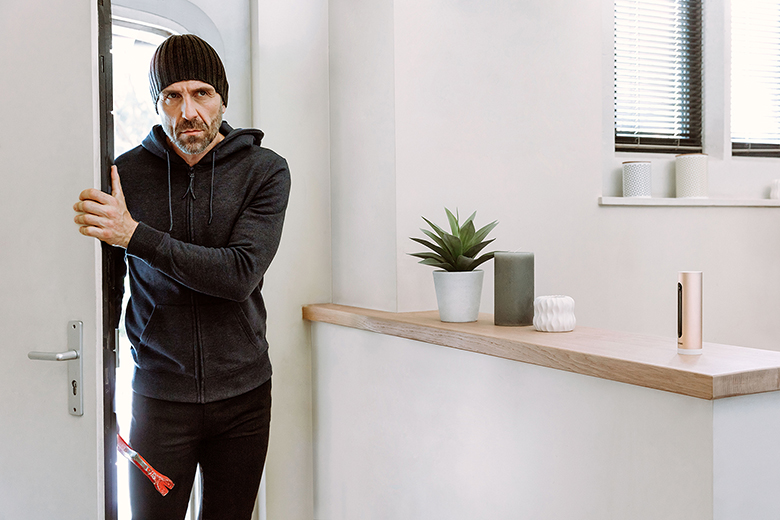
\includegraphics[width=8cm]{img/capitulo_3/intruso.jpg}
    \end{center}
    \caption{Ilustración de un ladrón}
    Fuente: Adaptada de Apellido, N. (2000) \textit{Nombre del libro}.
    Editorial o universidad que lo publicó.
    \label{fig:ejemplo}
\end{figure}
 
Hemos tratado de sintetizar estas posibilidades en función del tiempo de ausencia, estableciendo distintos casos con peculiaridades específicas en lo que se refiere a la seguridad y los riesgos que se afrontan, y empezando por exponer las medidas de protección más básicas y elementales que siempre se deberían tomar en consideración, tales como contratar un seguro para la vivienda (especificando algunos elementos importantes que figuran en toda póliza de esta índole para facilitar su elección y contratación).\\

\subsection{Ausencias cotidianas}
El primero de los casos supuestos es el más frecuente y cotidiano: las ausencias diarias de horas o minutos que brindan oportunidades a asaltantes atentos. Aquí, se tendrán en cuenta medidas de protección sencillas y sin complicaciones que cualquiera puede llevar a cabo apenas sin inversión alguna. Asegurar los cierres de los accesos a la vivienda, disimular las ausencias o evitar proporcionar información sobre nuestros hábitos son algunas de las medidas que se exponen para evitar intrusiones no deseadas en el hogar.\\
 
Como situación perteneciente a este grupo de supuestos, pero con riesgos añadidos y particularidades propias que obligan a prestarle una atención especial, se tratará aparte el caso de ausencias puntuales dejando en la vivienda a niños, personas mayores o dependientes sin nadie a su cargo. Evidentemente, aquí se tratarán amenazas y riesgos internos de la vivienda, tales como manipulaciones indebidas de instalaciones y componentes de especial peligrosidad, o la atención a emergencias que puedan suceder durante ausencias breves.\\

\subsection{Ausencias de termino medio}
Al salir de casa debemos saber si volveremos al cabo de pocas horas, de unos días o de semanas, ya que cada caso (como hemos comentado) presenta peculiaridades y riesgos específicos que tenemos que afrontar de distintos modos. El segundo supuesto, tras las ausencias cotidianas, será el caso de ausencias de pocos días, especialmente en fines de semana, puentes festivos y vacaciones cortas.\\
 
En estas situaciones convergen la necesidad de contar con alarmas y avisadores técnicos, con la de disponer de sistemas de alarma y dispositivos antiintrusión los cuales, como veremos, pueden ser de muy diversa índole.\\

\subsection{Ausencias prolongadas}
Las vacaciones y las estancias de cierta duración en lugares alejados de nuestras residencias habituales ofrecen oportunidades únicas a posibles asaltantes. No ofrecer información sobre nuestro paradero, tratar de evitar el efecto de vivienda vacía, contar con la supervisión regular de alguien de confianza en nuestra ausencia y mantener a buen recaudo bienes u objetos de valor serán, en estos casos, las principales prioridades (sobre todo en el caso de las segundas residencias, una cuestión que también consideraremos detalladamente como caso diferenciado).\\

\section{Situaciones de riesgo}
\subsection{Presencia de instrusos}

Referenciando a la figura \ref{fig:ejemplo}.
\begin{figure}[H]
    \begin{center}
        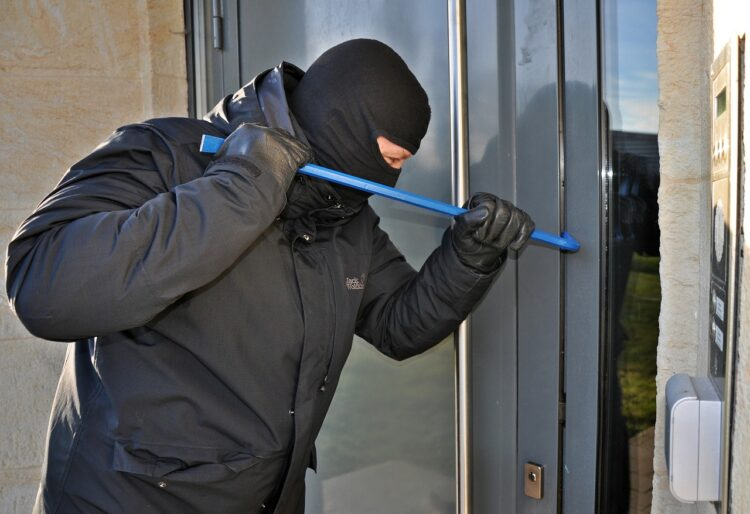
\includegraphics[width=8cm]{img/capitulo_3/burglar.jpg}
    \end{center}
    \caption{Ilustración de un ladrón}
    Fuente: Adaptada de Apellido, N. (2000) \textit{Nombre del libro}.
    Editorial o universidad que lo publicó.
    \label{fig:ejemplo}
\end{figure}

\subsection{Fuego y humo}
Referenciando a la figura \ref{fig:ejemplo}.
\begin{figure}[H]
    \begin{center}
        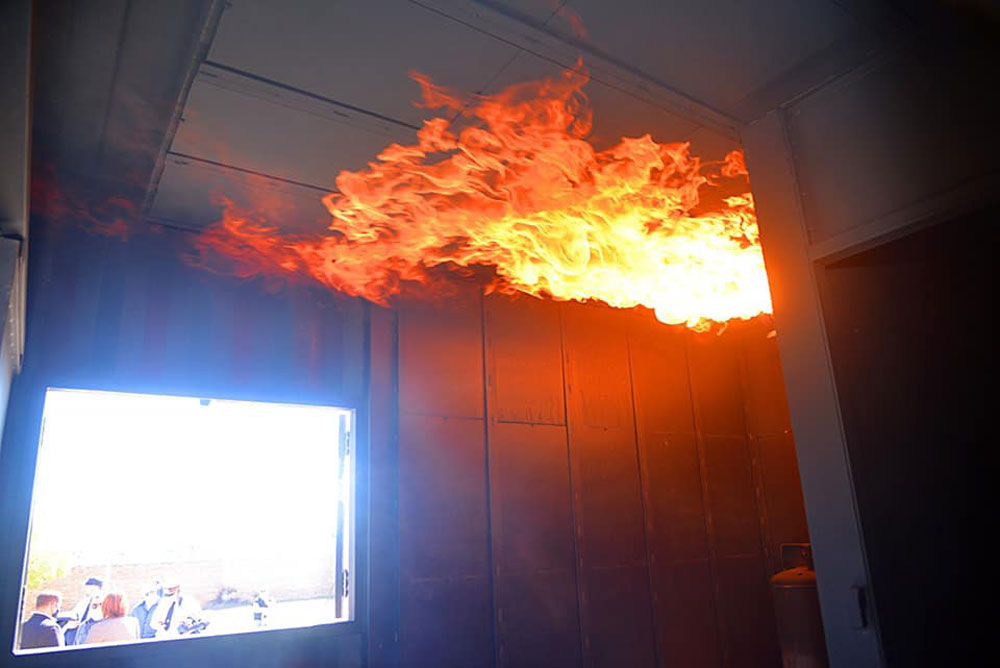
\includegraphics[width=8cm]{img/capitulo_3/fuego_en_interiores.jpg}
    \end{center}
    \caption{Ilustración de un ladrón}
    Fuente: Adaptada de Apellido, N. (2000) \textit{Nombre del libro}.
    Editorial o universidad que lo publicó.
    \label{fig:ejemplo}
\end{figure}

Referenciando a la figura \ref{fig:ejemplo}.
\begin{figure}[H]
    \begin{center}
        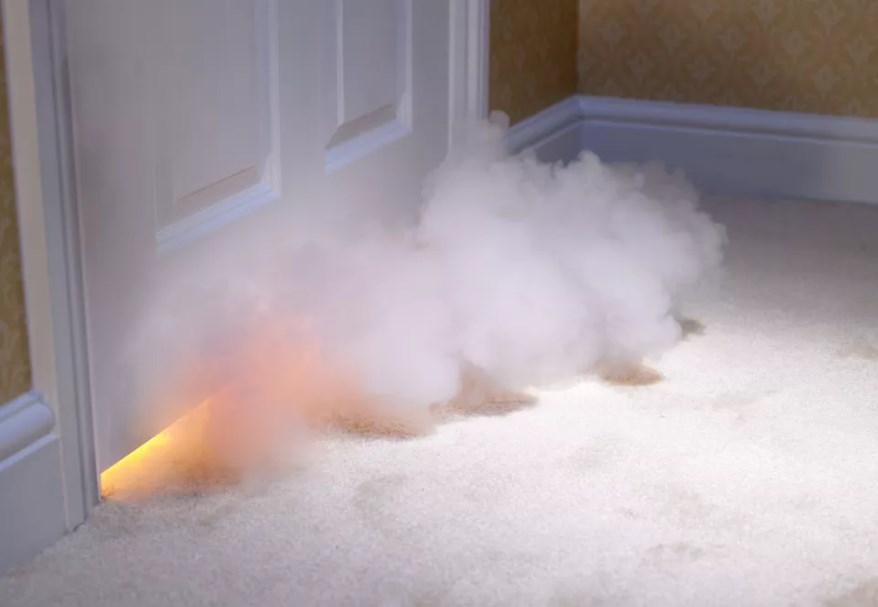
\includegraphics[width=8cm]{img/capitulo_3/fuego_en_el_cuarto.jpg}
    \end{center}
    \caption{Ilustración de un ladrón}
    Fuente: Adaptada de Apellido, N. (2000) \textit{Nombre del libro}.
    Editorial o universidad que lo publicó.
    \label{fig:ejemplo}
\end{figure}



\section{Sistemas de seguridad}
En el mercado, existen un sinfín de posibilidades al alcance para proteger nuestros hogares frente a casi cualquier tipo de amenaza, tanto interna como externa. Los más eficaces y eficientes, sin duda, son los sistemas electrónicos de seguridad, de los que ya hablamos detalladamente en la guía Hogares y negocios seguros\\

No obstante, sea cual sea la opción elegida a la hora de proteger nuestra vivienda durante ausencias más o menos prolongadas, debemos tener en cuenta los siguientes riesgos y amenazas:\\

Allanamientos, intrusiones y vandalismo: riesgos procedentes del exterior, que se pueden mitigar fácilmente instalando cierres de alta seguridad en los accesos a la vivienda, alarmas antiintrusión u otros mecanismos disuasorios.\\

Accidentes domésticos: riesgos procedentes del interior de hogar que pueden poner en riesgo la integridad física y/o moral de sus habitantes, tanto personas como mascotas, así como los bienes que contienen e incluso la misma infraestructura. Las alarmas técnicas (avisadores de fugas y escapes) y de emergencia son, para estos casos, los sistemas más adecuados para proteger una vivienda. También es preciso tomar las medidas oportunas para proteger los componentes más sensibles del hogar (instalaciones de suministros y otros elementos de riesgo) de manipulaciones indebidas, golpes y otro tipo de percances que pueden ocasionar accidentes o situaciones indeseables.

\subsection{Alarmas}
Referenciando a la figura \ref{fig:ejemplo}.
\begin{figure}[H]
    \begin{center}
        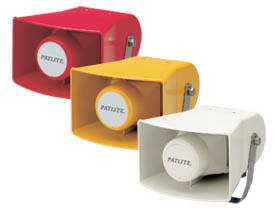
\includegraphics[width=6cm]{img/capitulo_3/alarmas.jpg}
    \end{center}
    \caption{Ilustración de un ladrón}
    Fuente: Adaptada de Apellido, N. (2000) \textit{Nombre del libro}.
    Editorial o universidad que lo publicó.
    \label{fig:ejemplo}
\end{figure}

\subsection{Sensores}
Referenciando a la figura \ref{fig:ejemplo}.
\begin{figure}[H]
    \begin{center}
        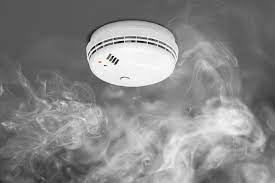
\includegraphics[width=6cm]{img/capitulo_3/sensor_de_humo.jpg}
    \end{center}
    \caption{Ilustración de un ladrón}
    Fuente: Adaptada de Apellido, N. (2000) \textit{Nombre del libro}.
    Editorial o universidad que lo publicó.
    \label{fig:ejemplo}
\end{figure}



\subsection{Cámaras}
Referenciando a la figura \ref{fig:ejemplo}.
\begin{figure}[H]
    \begin{center}
        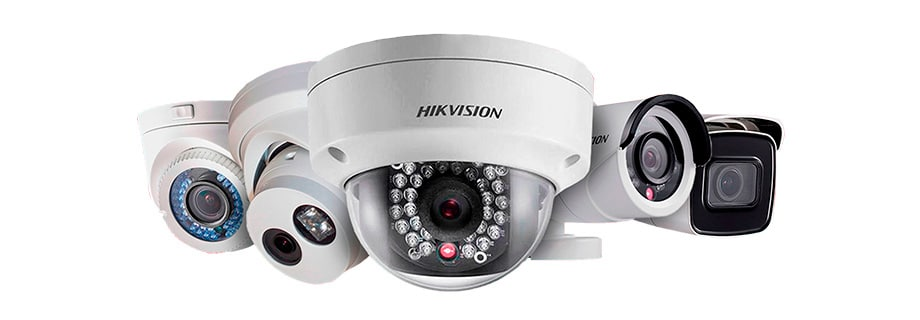
\includegraphics[width=8cm]{img/capitulo_3/camaras.jpg}
    \end{center}
    \caption{Ilustración de un ladrón}
    Fuente: Adaptada de Apellido, N. (2000) \textit{Nombre del libro}.
    Editorial o universidad que lo publicó.
    \label{fig:ejemplo}
\end{figure}

Referenciando a la figura \ref{fig:ejemplo}.
\begin{figure}[H]
    \begin{center}
        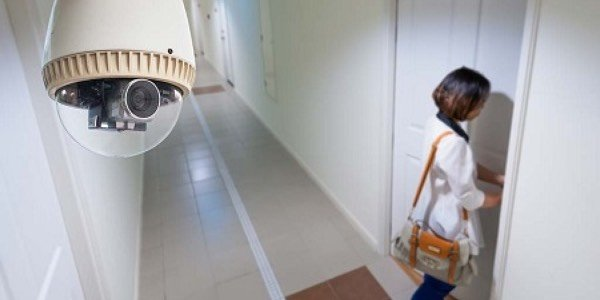
\includegraphics[width=8cm]{img/capitulo_3/camara_de_interiores.jpg}
    \end{center}
    \caption{Ilustración de un ladrón}
    Fuente: Adaptada de Apellido, N. (2000) \textit{Nombre del libro}.
    Editorial o universidad que lo publicó.
    \label{fig:ejemplo}
\end{figure}

Seguridad y vigilancia son aspectos que se requieren en todo el mundo; gobiernos, empresas, instituciones financieras, organizaciones de salud necesitan cierto grado de medidas de seguridad y como resultado se generó un dramático incremento en la demanda de aplicaciones de seguridad como por ejemplo video vigilancia, monitoreo y grabación de: fronteras, puertos, transporte, hogares, corporaciones, instituciones educativas, lugares públicos, edificios, etc.\\

La creciente demanda en el mercado de la vigilancia ha reducido costos en este tipo de sistemas, lo cual permitió que desarrolladores y fabricantes diseñen nuevas implementaciones de sistemas de video vigilancia agregándoles diversas capacidades dependiendo de la tecnología utilizada en su desarrollo. El mercado global de la video vigilacia fue avaluado en 42,94 billones de dólares en 2019 y esta proyectado alcanzar a los 144,85 billones de dólares hasta el 2027, registrando una taza de crecimiento anual compuesta del 14,6\% desde el 2020 al 2027.\\
